%コンパイル方法: opt+cmd+b → opt+cmd+v
\RequirePackage{plautopatch}

\documentclass[a4paper, 10pt]{ltjsarticle}


% マージン設定
\usepackage[top=20mm, bottom=20mm, left=20mm, right=20mm]{geometry}

% LuaLaTeX用日本語対応パッケージ
\usepackage{luatexja}
\usepackage{luatexja-fontspec}

% 必要なパッケージ
\usepackage{fontspec}
\usepackage{titlesec}
\usepackage{graphicx}
\usepackage{amsmath}
\usepackage{amssymb}
\usepackage[hidelinks]{hyperref}
\usepackage[english, japanese]{babel}
\usepackage{multicol} % 二段組用パッケージ
\usepackage{indentfirst}
\usepackage{tikz} % カスタム点線用
\usepackage{authblk} % 著者・所属パッケージ
\usepackage{here}
\usepackage{caption}
\usepackage{bookmark}

% \setmainfont[Ligatures=TeX]{Times New Roman}
% \setmainjfont[BoldFont=MS Gothic]{MS Mincho}

\renewcommand{\baselinestretch}{0.95}
\renewcommand{\labelenumi}{(\arabic{enumi})}

% セクション見出しのカスタマイズ
\titleformat{\section}
  {\fontsize{10pt}{10pt}}
  {\thesection.}
  {1em}{}

\titleformat{\subsection}
  {\fontsize{10pt}{10pt}}
  {\thesubsection}
  {1em}{}

\titleformat{\subsubsection}
  {\fontsize{10pt}{10pt}}
  {\thesubsubsection}
  {1em}{}

  \setlength{\parindent}{1em}
% \setlength{\belowcaptionskip}{1em} % キャプション下の余白を -10pt に設定


%section前に余白を作る
\titlespacing*{\section}{0em}{1em}{0em}
\titlespacing*{\subsection}{0em}{1em}{0em}
\titlespacing*{\subsubsection}{0em}{1em}{0em}

\pagestyle{empty}


\begin{document}

\setlength{\columnsep}{7.5mm}

\twocolumn[
    \begin{center}
        {\vspace{-1em}}

        {\fontsize{15pt}{15pt}\selectfont{アドホックネットワークについての研究(仮)}}

        {\vspace{1.5em}}

        {\fontsize{13pt}{13pt}\selectfont{}}
    \end{center}



    \begin{flushright}
      {\fontsize{11pt}{11pt}\selectfont{T5-17 末廣隼人\\}}
      {\fontsize{11pt}{11pt}\selectfont{指導教員 髙﨑和之}}
    \end{flushright}

    \vspace{1em}

    \thispagestyle{empty}
]

\section{研究背景}
% 自然災害、特に地震発生時に基地局の倒壊やネットワーク障害が生じたときに、
% その間に助けを求める人達の不安を少しでも拭うために一時的なネットワーク、
% アドホックネットワークの構築を行い少しでも多くの情報を共有できることを目的として研究を行った。\\
% 具体的には、被災エリアの中心に主となるノードを設置、その周りに携帯端末が保有するBluetoothなどでアドホックネットワークの構築おこうなう。
% このとき、全ての端末をアドホックに使用してしまうと、ルーティングが煩雑distribution化してしまうしまうため、
% アルゴリズムでメインとして使用する端末と接続が切れてしまった時の補助端末に分ける。その方法を第3章で述べる。

% 日本では多くの自然災害が発生しており、自然災害の中で一番恐れらている災害が地震であった。
% 昨年の石川県能登半島で発生した大地震では多くの死傷者がでてしまい、甚大な被害を被った。
% この災害では特に高齢者の人口が多く占めており、迅速な避難が難しかったり、

\section{理論}
\subsection{アドホックネットワーク}
アドホックネットワークとは、中央の管理者や既存のインフラストラクチャ(ルータやアクセスポイント等)を介さずに、端末(以降ノードと呼ぶ)同士が直接通信を行う一時的なネットワークのことである。
遠くのノードと通信を行うとき、隣接する他ノードを中継機として利用し、バケツリレーのようにデータを送信する「マルチホップ通信」技術を用いて通信を行う。%
\\ \indent 本実験では、低コスト、低消費電力でスマホに内蔵されているBluetoothを用いる。
特に、より消費電力が抑えられているBluetooth Low Energy(BLE)の接続距離である30mを想定してシミュレーションを行う。

\subsection{アドホックネットワークの技術的課題}
\subsubsection{隠れ端末問題}
隠れ端末問題とは、図1のようにノードAとCがノードBに対して通信を行うとき、ノードAとCはお互いの存在が隠れてしまい、
現在誰も通信を行なってないと思い込んで同時にノードBへと通信を行いデータが衝突してし壊れてしまう問題である。%
\begin{figure}[H]
  \centering
  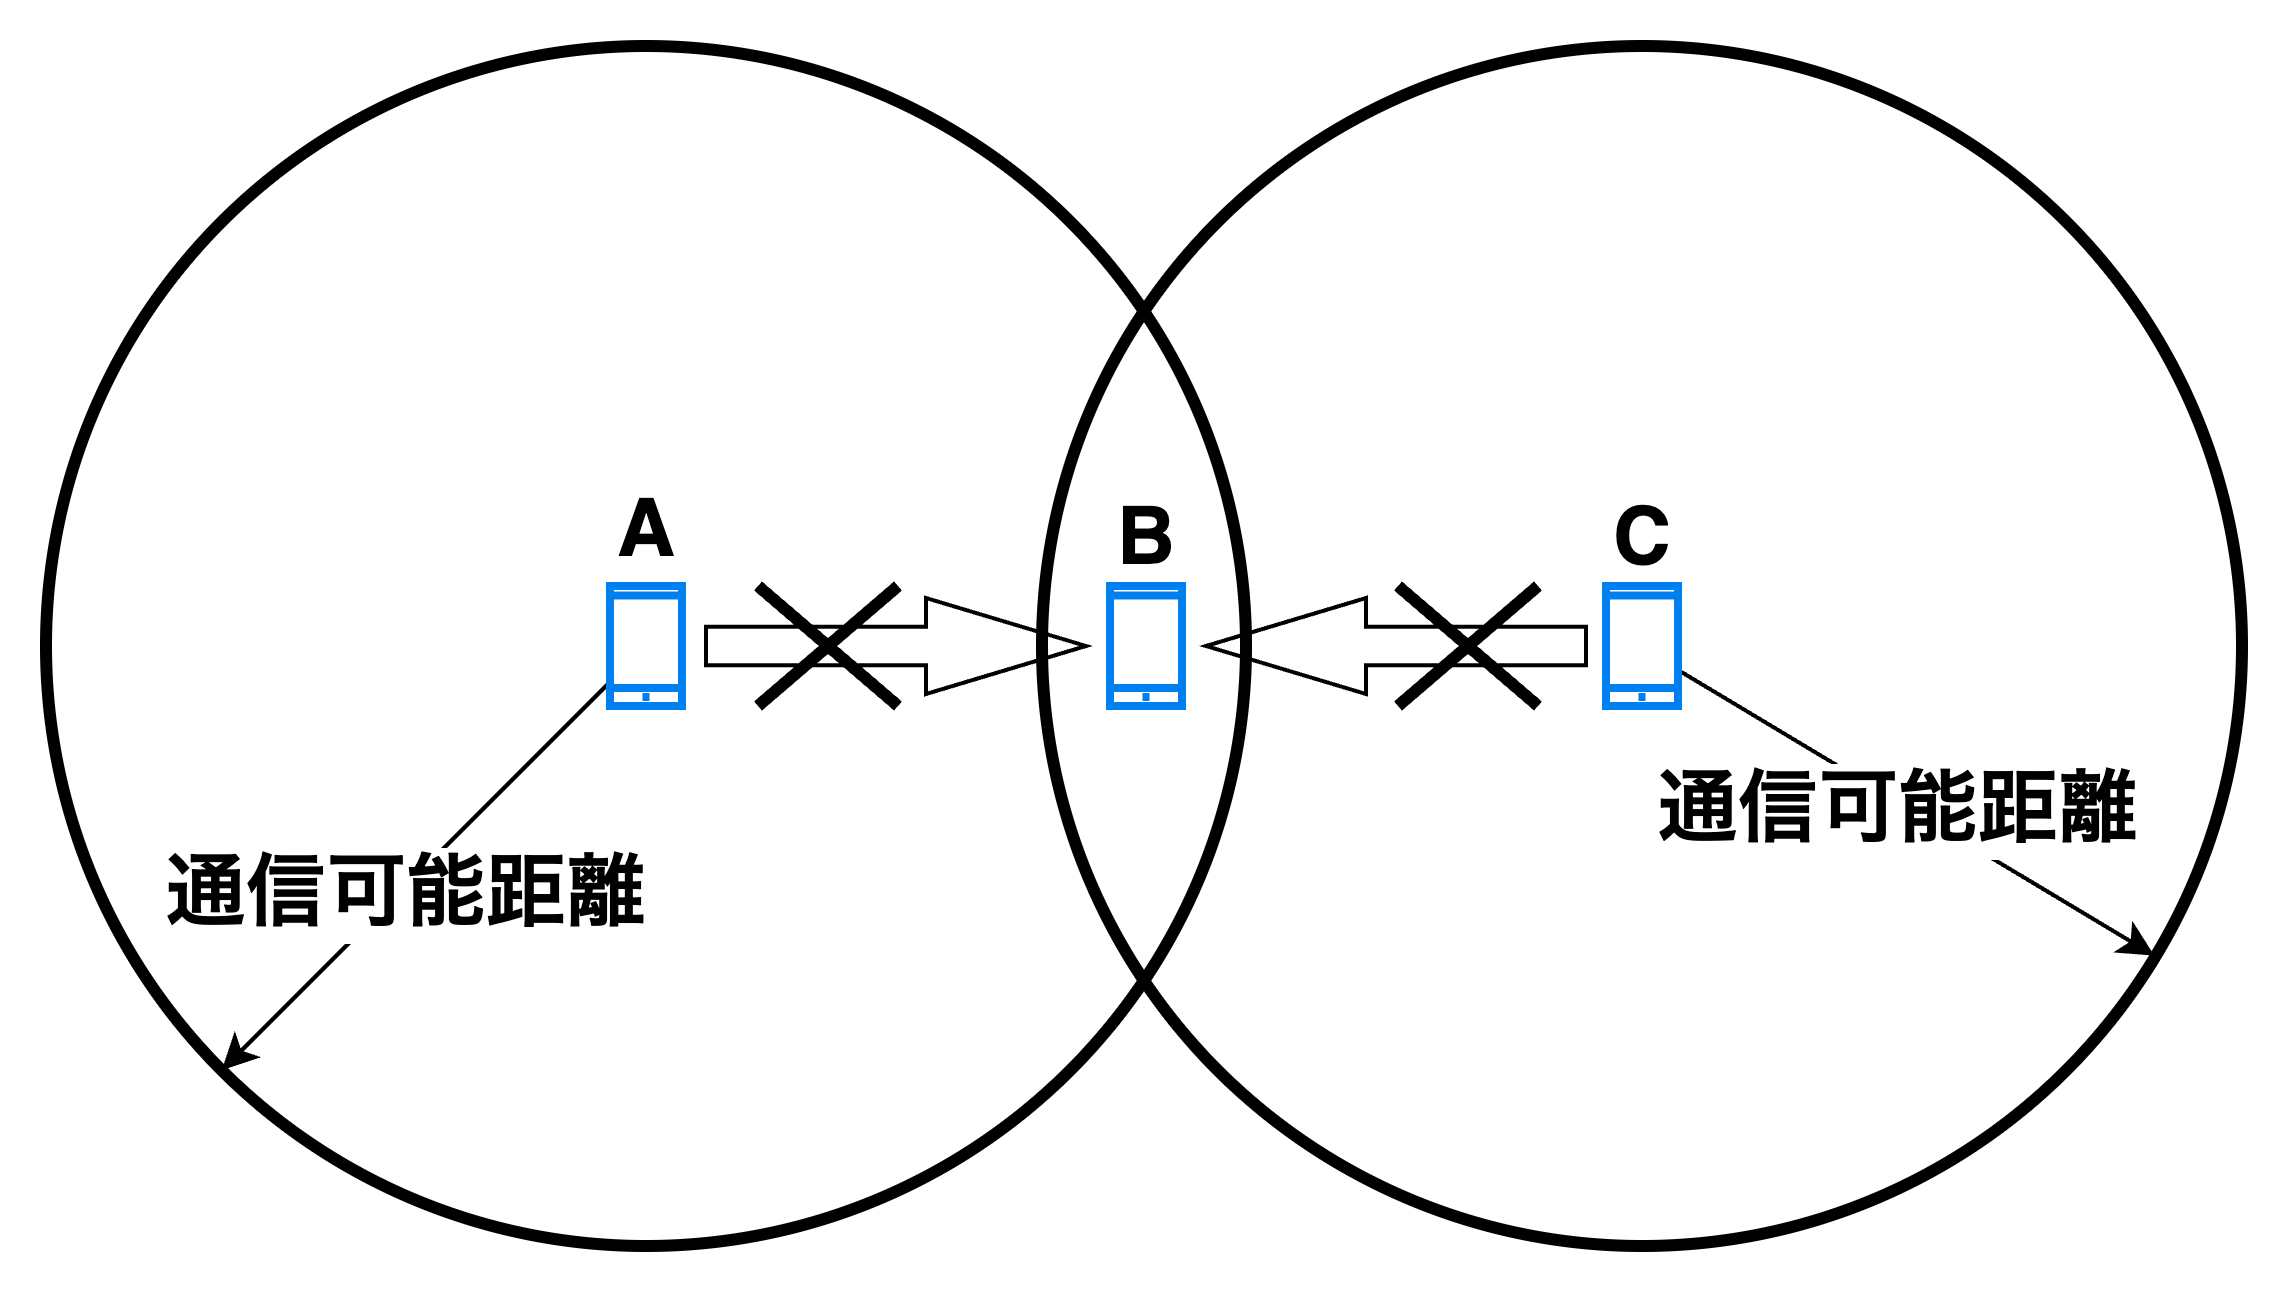
\includegraphics[width=70mm]{hidden_terminal_problem.png}
  \caption{隠れ端末問題}
\end{figure}

\subsubsection{さらし端末問題}
さらし端末問題とは、図2のようにノードAがDと通信を行なっているときノードBは端末Cと通信ができそうだが、
ノードAがDと通信を行なっているため周辺にいる他ノードは通信の抑制がされてしまい、
伝送速度や通信品質の低下が発生してしまう問題である。%
\begin{figure}[H]
  \centering
  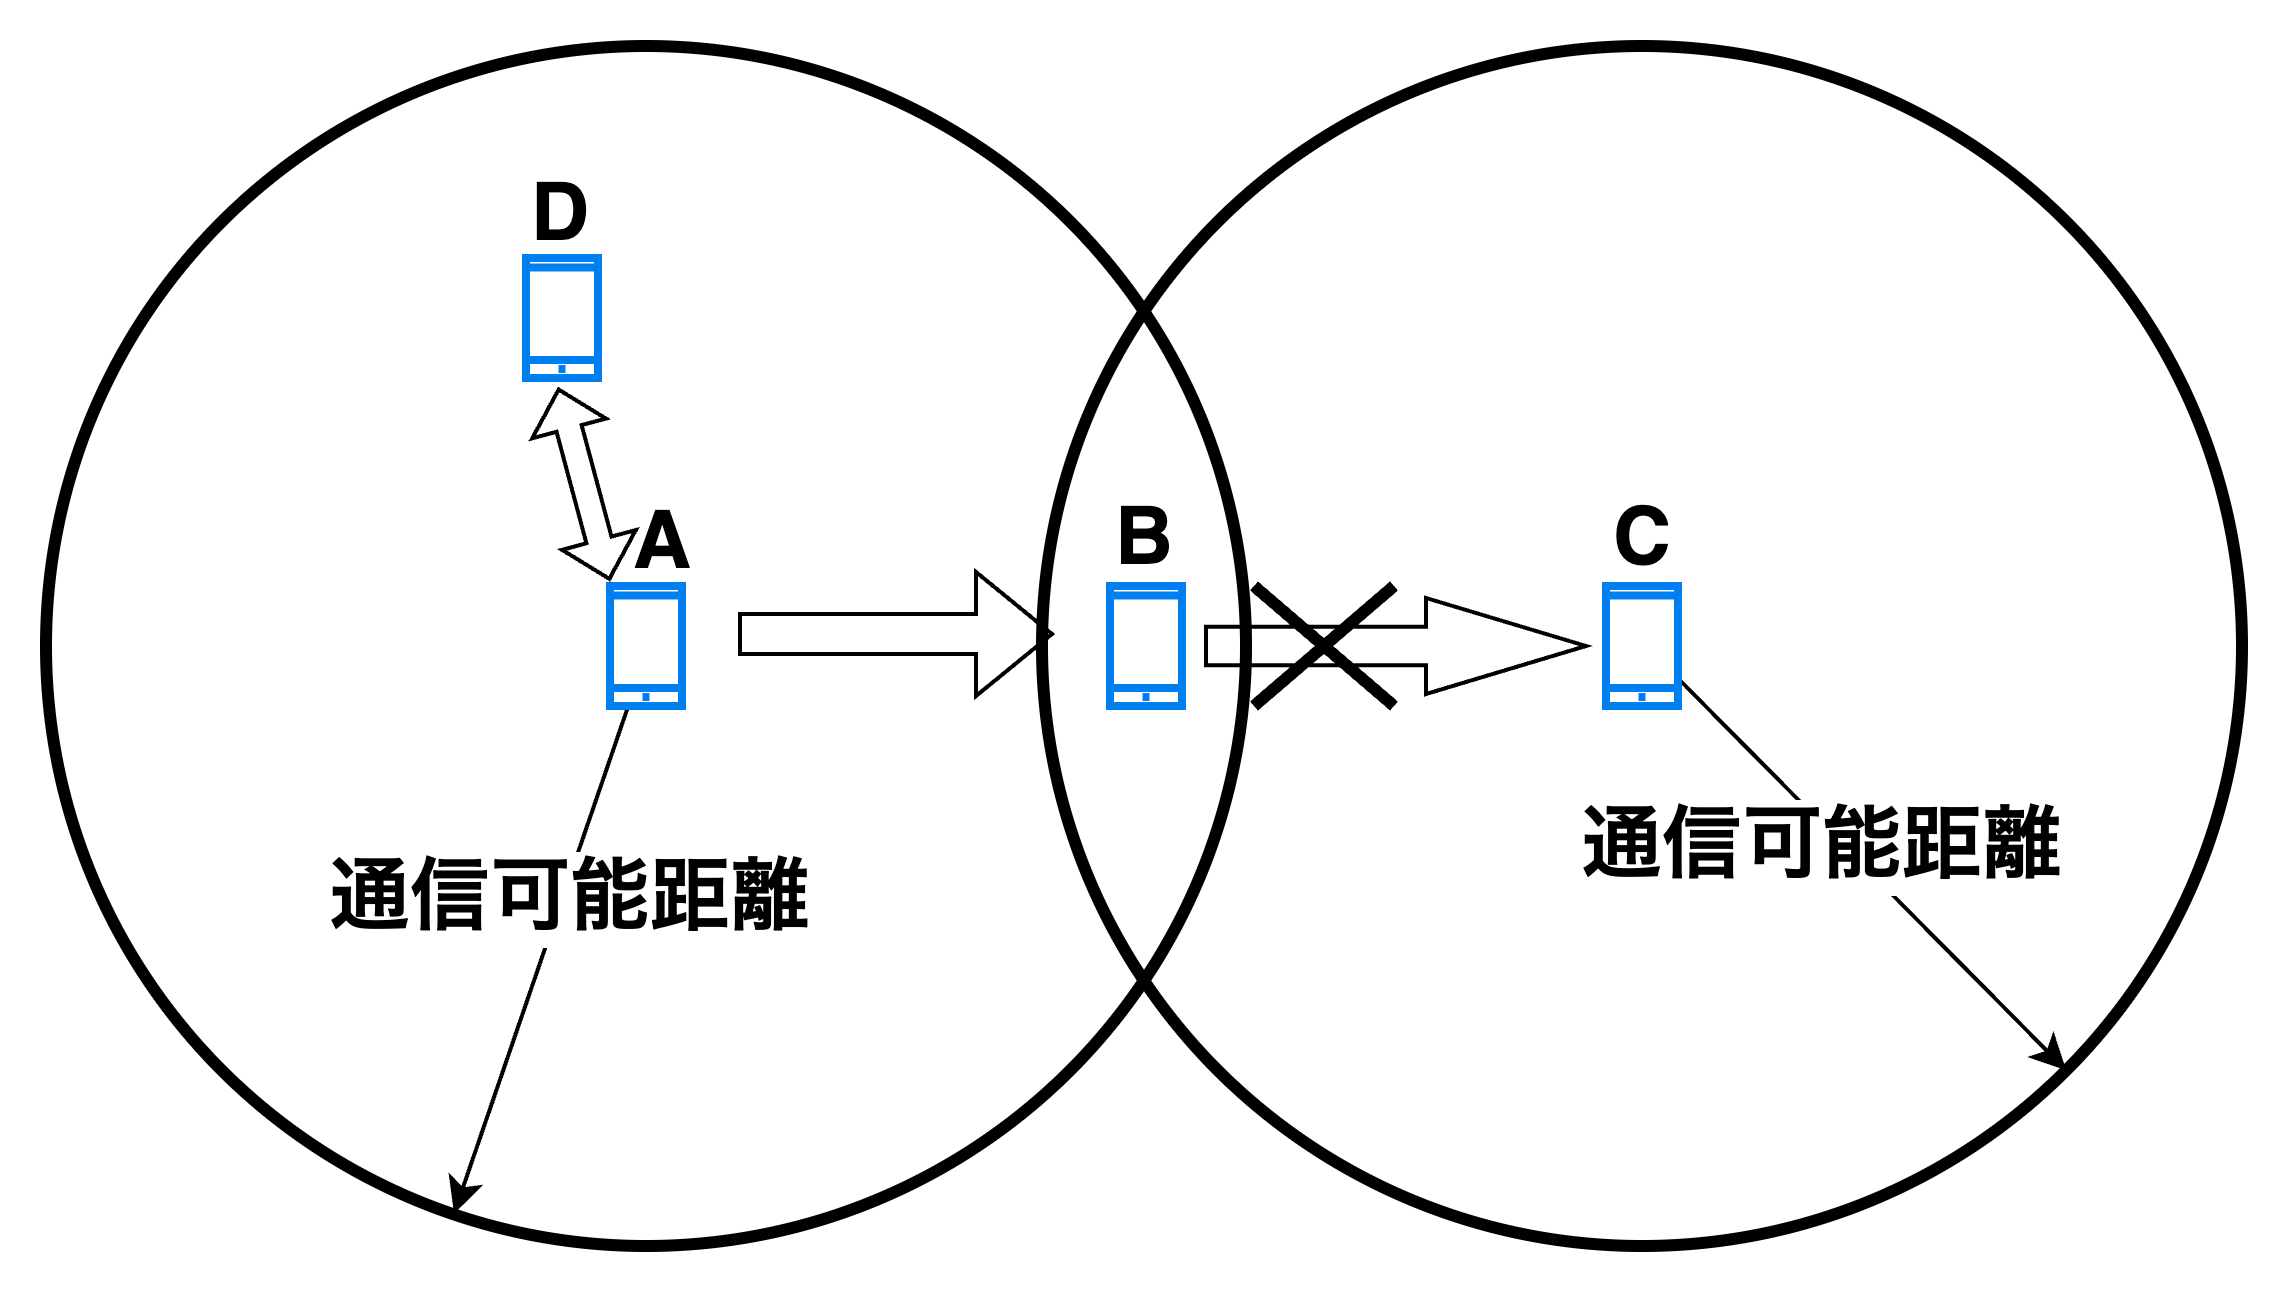
\includegraphics[width=70mm]{exposed_terminal_problem.png}
  \caption{さらし端末問題}
\end{figure}

\subsection{ルーティング制御方法}
各ノードと通信を行う際のルーティング方式について述べる。
ルーティング方式には大きく分けてリアクティブ型、プロアクティブ型、ハイブリッド型の3種類がある。
\begin{enumerate}
  \item \label{reactive} リアクティブ型\\ 通信要求を行った時に近くのノードとその場でデータのやり取りを行い経路を作成する。その場で経路を生成するため通信開始までに遅延が生じる。プロトコルとしてAODVやDSRなどがある。
  \item \label{proactive} プロアクティブ型\\ 近くのノード間で自身の情報をやりとし経路をあらかじめ作成するルーティング方式である。あらかじめ経路が作成されるため、通信開始までの遅延が短い。
  しかし、定期的にデータのやり取りを行うため電池の消費が早い。プロトコルとしてOLSRやTBRPFなどがある。
  \item ハイブリッド型\\ (\ref{reactive})、(\ref{proactive})の二つを組み合わせたルーティング方式である。プロトコルとしてはZRPなどがある。
\end{enumerate}

\section{提案手法}
\subsection{想定環境}
今回、経路生成にあたりノード数は日本の各都道府県の人口密度に持ち運びが便利なスマートフォンの所有率88.6\%\cite{スマホ保有率}を掛け合わせた数とする。%
用いる都道府県は人口密度が高い地域、低い地域と昨年被災した石川県珠洲市の3つの地域に対してシミュレーションを行う。

\subsection{提案手法-1}
$1\mathrm{km}^2$範囲内にノードをランダムに配置し、実際に被災が起きたことを想定し$1\mathrm{km}^2$の中心位置にあるノード
を災害対策本部の拠点とみなして、その位置からアドホックネットワークの構築を行う。構築方法の条件を以下のように設けた。
\begin{itemize}
  \item 接続半径内にいるノードの中から最も遠い(信号強度が通信品質に問題ない)ノードを選び接続を行う。
  \item 経路のループが起きないようにパラメータs(任意の数)とホップ数をmodで計算した時0になったノードとの接続を遮断する。
\end{itemize}

\subsection{提案手法-2}
次に、電柱の本数分加えたシミュレーションを行った。また、提案手法-1と同様に$1\mathrm{km}^2$の中心位置から構築を行うが、
新たに追加した電柱のノードに対しての条件を設けた。
\begin{itemize}
  \item 
\end{itemize}

\section{結果}

\section{まとめ}

\begin{thebibliography}{9}
  \bibitem{スマホ保有率} https://www.soumu.go.jp/johotsusintokei/whitepaper/ja/r04/html/nd238110.html, 総務省, 「通信利用動向調査」 
\end{thebibliography}

\end{document}
